\documentclass{article}[18pt]
\title{Business Plan}
\author{mbkb74}
\usepackage[margin=1in]{geometry}
\usepackage{pdfpages}
\usepackage[toc,page]{appendix}
\usepackage{multirow}
\usepackage{tabularx}
\usepackage{array}
\pretolerance=10000
\begin{document}
\maketitle
	
\tableofcontents
\newpage
\section{Executive Summary}
Menuscan is an app used to scan menus to give more detail on certain dishes, and to hide items with certain allergens in them.\\
\\
Menuscan can start without contact with businesses, using computer vision on the menus to get all the information it needs. However, as Menuscan grows we will gain sponsorship from businesses to promote certain deals in an overlay on their menu.\\
\\
Menuscan can also have a long term goal of using all the data from the scanned menus, combined with location to provide a search feature to allow you to see where nearby serves certain dishes.\\
\\
Another source of revenue would be normal advertising within the app, there are no plans to have any cost to the user of using the app.
\section{Business Details}
I am a one person developer aiming to produce the app at a low cost, the app will combine computer knowledge and processing with physical menus to give more information to people at restaurants. The target market for this business is everyone visiting restaurants and this is a for profit enterprise. The app should take 4 months to get an initial design and then continued development to add new features. This is a digital business in the technology sector, but it also has overlaps with the food industry. The longer term vision for this company is to continue developing features and increasing the reach of the company to allow it to grow.
%\textbf{Who I am} - A one person developer aiming to produce the app at a low cost\\
%\\
%\textbf{What are we going to do} - Produce an app to combine computer knowledge with physical menus\\
%\\
%\textbf{What do we have to offer} - Additional knowledge to that presented on a physical menu\\
%\\
%\textbf{Target Market} - Everyone visiting restaurants\\
%\\
%\textbf{What type of enterprise is it?} - A for profit enterprise\\
%\\
%\textbf{Timescale} - The app should take 4 months to get an initial design out there, and then continued development will add features\\
%\\
%\textbf{Type of business and sector} - Digital business in the technology sector, with overlap into the food industry\\
%\\
%\textbf{Longer term vision} - Continued feature development to allow all information on menus to be easier and more accessible.
\subsection{Value Proposition}
This business is different as nothing like this currently exists on the market. The current closest competitor would be the customer using google to search the items on the menu, but the increased friction of this process would allow my business to thrive.\\
\\
This offering uses the ease of scalability within the technology sector to allow it to grow quickly and internationally. The speed of production for a product in the technology industry will allow me to start generating revenue after only 4 months, a huge advantage for the company. The ease to which updates can be provided to technological products is also an advantage as even in its infancy the app may be attractive to customers because they know that there will be continuous improvements.\\
\\
This product offers customers an easier understanding of the items on the menu. It also provides restaurants with an opportunity to advertise with us, so that the view the customer sees would promote certain deals. As features develop there may be other ways that we could attract restaurants, for example by scanning menus we are able to get all the menu details of restaurants. This data could then be used in a searchable form so that customers could search for a certain dish and the restaurants what serve it would be shown, with promoted restaurants at the top.\\
\\
We may consider applying for a patent for some of our intellectual property, but being first to market should give us enough advantage over any small company, the only concern would be if a large company created an imitation.
%
%\textbf{What makes my business different} - Nothing like this exists on the market, the current closest competitor would be people googling the items on the menu, but the increased friction of this allows my business to thrive.\\
%\\
%\textbf{How what you are offering relates to key features of your industry or sector} - This offering uses the ease of scalability within the technology sector to allow it to grow quickly. The speed of production for a product in the technology sector will also be an advantage when it comes to financials\\
%\\
%\textbf{What benefits does your product/service offer?} - Allows users to easier understand the items on menus\\
%\\
%\textbf{Why would customers buy/commission/subscribe to you?} - Businesses would advertise with us to better promote their deals, and possibly their whole restaurant in the long run.\\
%\\
%\textbf{How will you develop your products or services} - One main area of development is using the scans of menus combined with the locations to allow for people to search for certain items and see where nearby serves them. This would also allow for a new revenue stream as companies could pay to be placed at the top of the list.\\
%\\
%\textbf{Intellectual property} - We may consider applying for a patent, but being first to market should give us enough advantage, with the only worry being if a large company imitates this idea.
\subsection{Business Model Canvas}
This can be found in appendix \ref{appendix:BMC}
\subsection{SWOT Analysis}
This can be found in appendix \ref{appendix:SWOT}. Overall I think that the company passes the SWOT analysis as no critical flaws have been found with the business.
\section{Industry and Market analysis}
The overall macro context in respect to how receptive the market would be to my venture is that there has been an increased demand in the restaurant industry with products such as Just Eat and Deliveroo, however there hasn't been as much growth in the sit in restaurant sector, so this new development could help revitalize that. But we do need to be aware of the lack of growth in restaurants as a possible problem with our business as they may be going out of fashion.\\
\\
Our company spans two industries, the technology industry and the restaurant industry. The technology industry is highly competitive, but there is also a lot of growth and high demand. The restaurant industry is competitive, but is much more stagnant than the technology industry and is less receptive to disruption.\\
\\
The market we are in has plenty of room for growth as there is no other company offering the exact service we provide. The closest competitor would be people googling items on the menu, but with the better ease of use, alongside extended functionality, our company should be able to thrive.\\
\\
Into the future we hope that the company is successful in the market, allowing for further development as revenue increases. Developing more features could allow for additional revenue streams, alongside providing increased functionality to the user, making the app more appealing.

%\textbf{What is the overall macro context like in respect to receptiveness for your venture} - There is increased demand in the restaurant industry with product such as Just Eat and Deliveroo, but there hasn't been much development in the sit in restaurant sector, so this new development could help to revitalize that.\\
%\\
%\textbf{What is the industry like} - The technology industry is highly competitive, but also with very high demand. The restaurant industry is competitive, but not growing as fast as the technology industry.\\
%\\
%\textbf{What is your market like} - The market has plenty of room for growth, which will allow for my company to be successful\\
%\\
%\textbf{Competitors} - There is no other company offering the exact service we provide. The closest competitor would be people googling the items on the menu, but the increased ease of use, alongside extended functionality will allow our company to thrive.\\
%\\
%\textbf{The future} - Hopefully this company will start to take off, allowing for further development as revenue increases. Developing more features could allow for additional revenue streams, alongside providing increased functionality for the user, making the app more appealing
\section{Customers and value proposition}
Our target customers for this product is all customers going to restaurants. This provides a very large client base. Using the scalability and ease of distribution of products in the technology sector we will be able to make this initially available to all English-speaking people. We will interact with these customers through official product pages, support contacts, through the app and through social media channels.

%\textbf{Customer Segments} - This product will appeal to all customers going to restaurants, which provides a very large client base. Using the scalability of products in the technology sector this will initially be available to all English-speaking people\\
%\\
%\textbf{What kind of relationships will you have with them} - We will interact with customers through official product pages, support contacts, through the app and through social media channels.

\subsection{PESTEL Analysis}
This can be found in appendix \ref{appendix:PESTEL}. There are no obvious issues found here, and we are happy to continue with the venture after doing this analysis.
\section{Marketing strategy}
We plan to use a range of activities in order to promote our service, this will range from social media communications to a variety of advertising through apps, on the web, on billboards and through influencers.\\
\\





%\textbf{What specific activities you intend to use to promote and sell your products and services}
%\begin{itemize}
%	\item Social media communications
%	\item Advertising in apps and on the web
%	\item Advertising on billboards
%	\item Advertising through influencers
%\end{itemize}
\begin{center}
{\renewcommand{\arraystretch}{2}
\begin{tabular}{| m{0.2\linewidth} |m{0.8\linewidth}|}
\hline
\textbf{Price}&This will appeal to customers as it is free\\
\hline
\textbf{Product}&
\begin{itemize}
	\item This satisfies customers who don't understand items on a menu
	\item It has the feature of showing images and descriptions of items on a menu
	\item The customer will use it on the app in restaurants
	\item It is called MenuScan
	\item It is differentiated as there is not another product on the market that does this
\end{itemize}\\
\hline
\textbf{Promotion}&
\begin{itemize}
	\item Promotion can be done through many channels
	\begin{itemize}
		\item Online
		\item Billboards
		\item TV
	\end{itemize}
	\item There isn't a lot of seasonality in the market, however targeted advertisements around Mother's Day, Father's Day and Valentines could prove useful
\end{itemize}\\
\hline
\textbf{Place}& This product will be available on the Android and iOS app stores\\
\hline
\end{tabular}}
\end{center}
\section{Operations plan}
The product will be produced in WeWork offices, these are £250 per month for a hotdesk and so are cheaper than an office, alongside coming with all maintenance etc. covered. No more equipment will need to be purchased as the products can be produced using my current computers. The logistics for the product will be simple as it is a digital product, so it can be uploaded to app stores and instantly distributed to customers around the world. The production process will be done solely by me in order to reduce costs, I will start on development of the Android app due to the larger market share and that should be complete in 4 months, and then the iOS app should take a further 4 months.\\
Due to my knowledge of IT systems no external people will be needed to help set up the IT systems. In terms of my capability, as I am a sole person, I can only work on one project at once, increasing the team size would allow for simultaneous development, but I haven't deemed the additional cost worth it in order to speed up production. As this is a digital product no supply chain will be needed, further cutting costs. There will be additional costs for accounting and marketing as I do not have the necessary skills. The calculated development lead time will be 4 months.



%\begin{itemize}
%	\item Location
%	\begin{itemize}
%		\item This will be produced in WeWork offices
%	\end{itemize}
%	\item Equipment/machines/premises
%	\begin{itemize}
%		\item The product will be produced using my current computers so will not require any more equipment investment
%	\end{itemize}
%	\item Logistics
%	\item Production process
%	\begin{itemize}
%		\item The app development will be carried out solely by me, starting on Android due to the larger market share and then moving on the the iOS app
%	\end{itemize}
%	\item IT
%	\begin{itemize}
%		\item Due to my knowledge of IT systems no additional IT will need to be set up
%	\end{itemize}
%	\item Team's capability
%	\begin{itemize}
%		\item As I am a sole person, I can only work on one project at once. Increasing to two people would allow the iOS and Android app to be developed simultaneously, but I have considered this and it is not worth the additional cost.
%	\end{itemize}
%	\item Suppliers and supply chain
%	\begin{itemize}
%		\item No physical product will be required so a supply chain will not be needed
%	\end{itemize}
%	\item Outsourcing for expertise
%	\begin{itemize}
%		\item Outsourcing for accounting and marketing will be used
%	\end{itemize}
%	\item Development lead times
%	\begin{itemize}
%		\item There is a 6 month development lead time
%	\end{itemize}
%\end{itemize}
\section{Management team and company structure}
The company will start very small, with only me as a permanent employee and outsourcing marketing and accounting to temporary workers.\\
\\
I have expertise in Programming and am enrolled in a Computer Science Degree, so I have the capability to make the app, but I do not have the skills for marketing or accounting so those will be outsourced.
\section{Financing and Financial Projections}
The table for the financials can be found in appendix \ref{appendix:Financials}. These show that the breakeven point will be reached in 11 months. Initial capital of £5664 will be needed to sustain the company before it starts making profit.
\section{Risk and Strategic options}
One of the risks to the company would be competitor action. Against another start-up we would have the first mover advantage and so I believe that our market penetration and industry contacts gained over that time would allow us to succeed and the imitator company fail. However, against a larger company, their significantly larger resources for things such as marketing and development would allow them to succeed over us. If this was to happen I believe that it would be best to change our business model somehow to fit in alongside them.\\
\\
Another risk is commercial issues, such as not getting enough revenue. This would happen if companies didn't take to sponsoring us as much as expected, if this was to happen then we would have to find additional funding to give us time to grow and so become more attractive to sponsors. This additional funding would be best sought from venture capital firms, but if in a small amount could also be sought as a loan from a bank.\\
\\
If we were to have issues with operations, such as slower production than expected, then we would need additional funding to continue development, this would be sought in the same way as for commercial issues.\\
\\
While I am the sole employee there will be no issues, as long as there is enough money for a living wage. When it comes to expanding the business we would hire employees with skill in proportion to the amount of money we are able to give them. We would potentially hire temporary workers to start with to have increased flexibility.\\
If there was any disaster with the offices, as we are working out of WeWork offices we would be compensated and would be able to move to alternate offices without having to deal with any of the issues. If there was a disaster regarding data, all the code would be regularly backed up and so could not be lost.
%\begin{itemize}
%	\item Competitor action
%	\begin{itemize}
%		\item Against another start-up we would have the first mover advantage and so our market penetration and industry contacts would allow us to succeed
%		\item Against a larger company they would have significantly larger resources for things such as marketing and development, so we may have to change our business model to fit in around them
%	\end{itemize}
%	\item Commercial issues
%	\begin{itemize}
%		\item If companies don't take to sponsoring as much as we expected then we will have to find additional funding in order to continue operations. This could be sought from venture capital firms.
%	\end{itemize}
%	\item Operations
%	\begin{itemize}
%		\item If production was slower than on schedule then we would need to gain additional funding to continue development, again this could be sought from venture capital firms.
%	\end{itemize}
%	\item Staff
%	\begin{itemize}
%		\item While I am the sole employee there will be no employee issues, when it comes to expanding the business we can seek skilled employees corresponding to the amount of money we have available to give them as a salary.
%	\end{itemize}
%	\item Fire, flood, other disasters
%	\begin{itemize}
%		\item All development will be backed up using the 3-2-1 method, and by using offices from WeWork, if there is a disaster at the offices then we could just move to one of their other locations
%	\end{itemize}
%\end{itemize}
\section{Key Milestones}
\begin{enumerate}
	\item Start Development
	\item Launch
	\item First Sponsor
	\item Breakeven Point
	\item Hiring another employee
\end{enumerate}
\begin{appendices}
\appendix
\section{Business Details}
\subsection{Business Model Canvas}
\label{appendix:BMC}
\begin{center}
{\renewcommand{\arraystretch}{2}
\begin{tabular}{| m{0.2\linewidth} |m{0.8\linewidth}|}
\hline
Value Propositions&
\begin{itemize}
	\item Find out what the items on a menu are
	\item Allows restaurants to promote deals when their menus are scanned
\end{itemize}\\
\hline
Key Activities&
\begin{itemize}
	\item Service development and maintenance
	\item Marketing and ads
	\item Operations
\end{itemize}\\
\hline
Key Resources&
\begin{itemize}
	\item Tech Platform
	\item Talented employees
	\item Brand
\end{itemize}\\
\hline
Key Partners&
\begin{itemize}
	\item Computer Vision Companies
	\item Image provision companies
	\item Investors
	\item Dictionary/description companies
\end{itemize}\\
\hline
Customer Segments&
\begin{itemize}
	\item People who don't know what an item on a menu is
\end{itemize}\\
\hline
Customer Relationships&
\begin{itemize}
	\item Review of result system
	\item Social Media Channels
	\item Official Product Pages
	\item Support contact
\end{itemize}\\
\hline
Channels&
\begin{itemize}
	\item The app
\end{itemize}\\
\hline
Cost Structure&
\begin{itemize}
	\item Software development
	\item Business expenses
	\item Image royalties
\end{itemize}\\
\hline
Revenue Streams&
\begin{itemize}
	\item Ads
	\item Restaurants pay to have their deals shown when the menu is scanned.
\end{itemize}\\
\hline
\end{tabular}}
\end{center}

\subsection{SWOT Analysis}
\label{appendix:SWOT}
\begin{center}
{\renewcommand{\arraystretch}{2}
\begin{tabular}{| m{0.2\linewidth} |m{0.8\linewidth}|}
\hline
Strengths&
\begin{itemize}
	\item First to the market with this idea
	\item Give more details on menus more than anyone else
	\item Can draw upon personal programming expertise
	\item People in the market see us being free as a strength
\end{itemize}\\
\hline
Weaknesses&
\begin{itemize}
	\item Improve feature set
	\item Avoid poor user experience leading to a slow experience
	\item Avoid the interface becoming so cluttered with ads it is difficult to use
	\item People in the market will see our small size as a weakness
	\item Bad customer relations could lose sales
\end{itemize}\\
\hline
Opportunities&
\begin{itemize}
	\item Improve feature set
	\item Avoid poor user experience leading to a slow experience
	\item Avoid the interface becoming so cluttered with ads it is difficult to use
	\item People in the market will see our small size as a weakness
	\item Bad customer relations could lose sales
\end{itemize}\\
\hline
Threats&
\begin{itemize}
	\item A larger company could see our app idea and could potentially easily replicate it
	\item If development takes longer than expected then cash flow could be a problem
\end{itemize}\\
\hline			
\end{tabular}}
\end{center}
\newpage
\section{Customers and Value Proposition}
\subsection{PESTEL Analysis}
\label{appendix:PESTEL}
\begin{center}
{\renewcommand{\arraystretch}{2}
\begin{tabular}{| m{0.2\linewidth} |m{0.8\linewidth}|}
\hline
Political& There are no government policies which could impact the company\\
\hline
Economic&With economic growth more people would visit restaurants, and so the app would have more use\\
\hline
Social&	A young and technologically apt group of customers would be best for using this product. Luckily there is a social trend towards increased technological awareness\\
\hline
Technological&	As the technological landscape changed we will have to change features, but in its current state the app seems to fit in well\\
\hline
Environmental&The app uses no resources so there are not environmental concerns with that. Using a co-working space is very environmentally friendly.\\
\hline
Legal&We will hire an external legal expert to ensure that everything is done to code, there doesn't seem to be any large legal issues that would prevent the company's existence.\\
\hline
\end{tabular}}
\end{center}

\section{Financials}
\label{appendix:Financials}
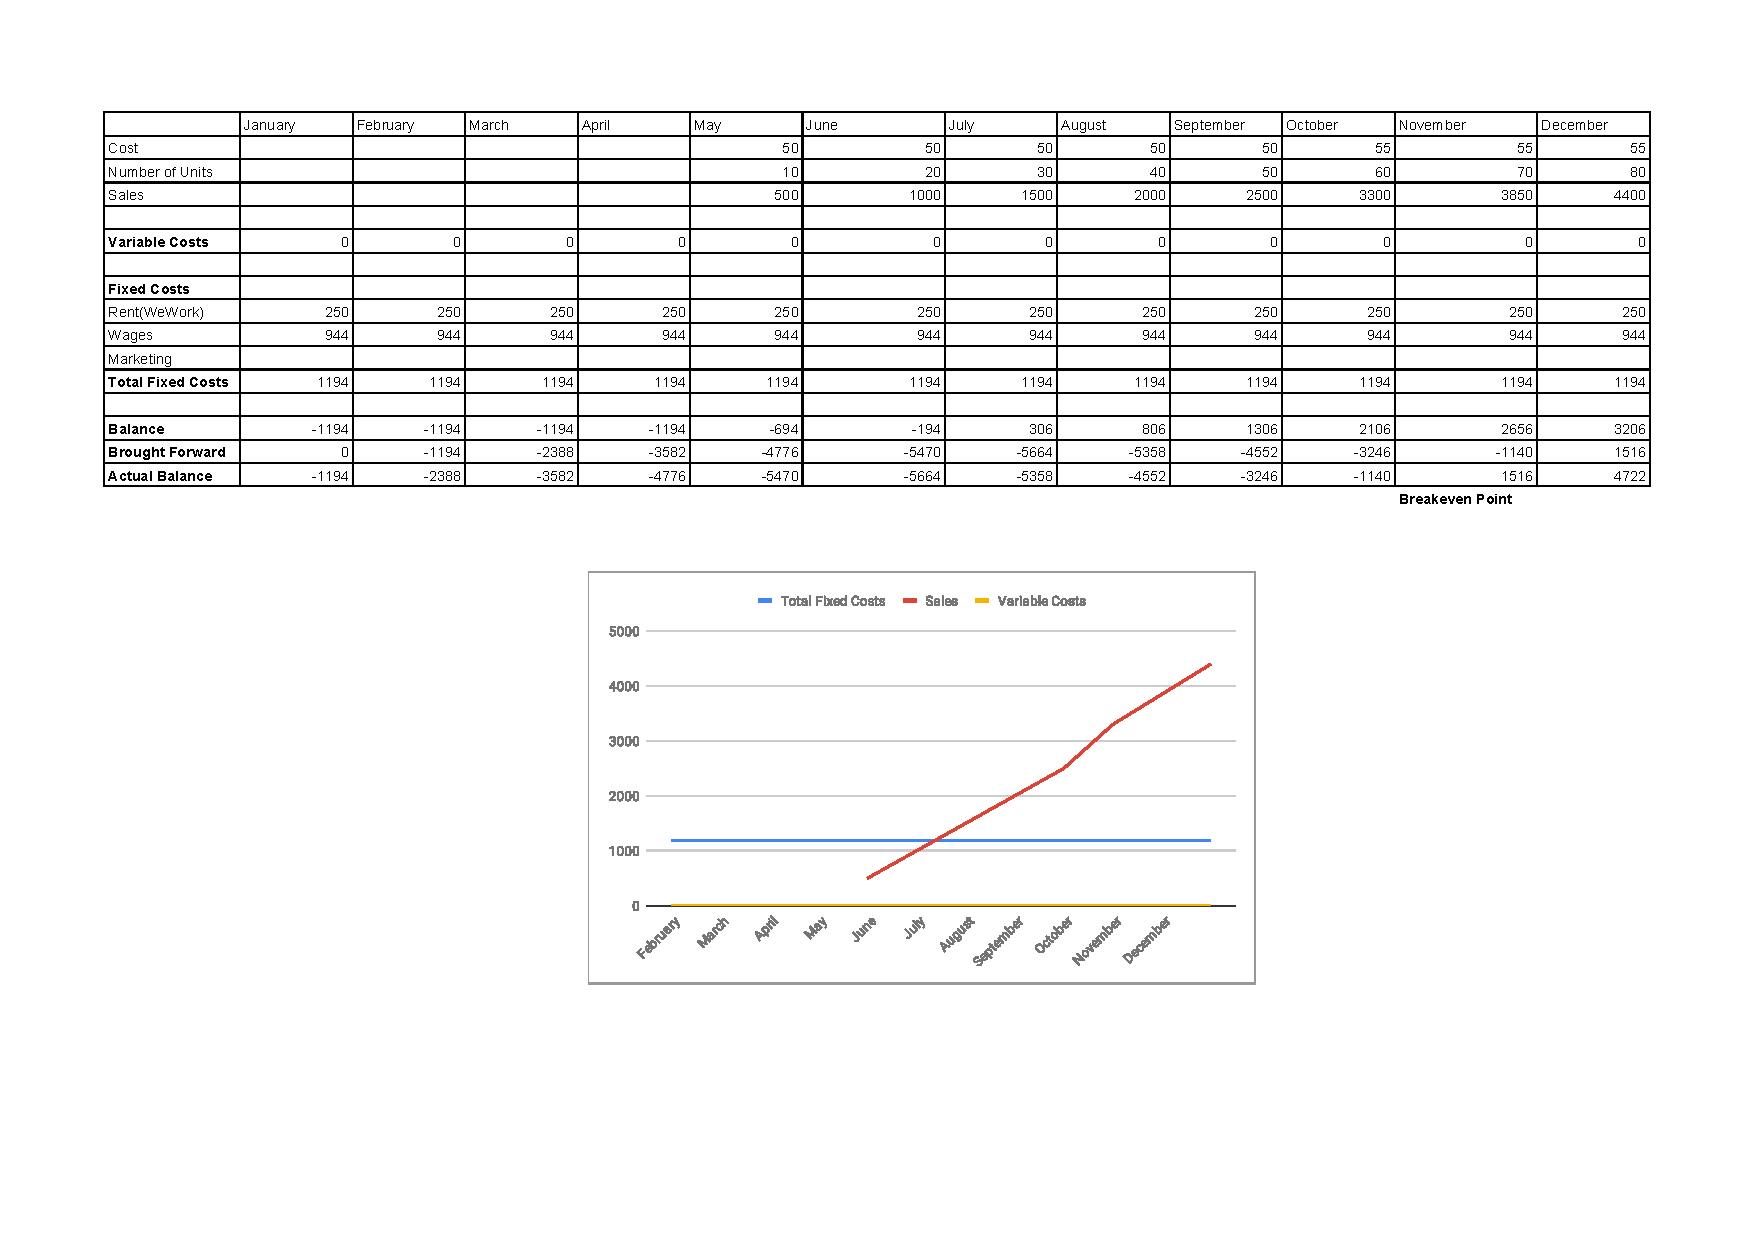
\includepdf[landscape=True]{Financial}
\end{appendices}
\end{document}